\documentclass[final,5p,times,twocolumn,authoryear,11pt,nonatbib]{elsarticle}

% ============================================================
% CONFIGURACION GENERAL
% ============================================================

% ============================================================
% PAQUETES DEL PROYECTO
% ============================================================
% Agregar aqui paquetes compartidos por todas las secciones.

\usepackage[spanish]{babel}
\addto\captionsspanish{\renewcommand{\tablename}{Tabla}}
\usepackage[utf8]{inputenc}
\usepackage[T1]{fontenc}

\usepackage{amsmath}
\usepackage{amssymb}
\usepackage{graphicx}
\usepackage{booktabs}
\usepackage{threeparttable}
\usepackage{caption}
\usepackage{csquotes}
% APA 7 con autor-año. La opción natbib mantiene disponibles \citep y \citet.
% elsarticle se carga con nonatbib para evitar dos gestores bibliográficos.
\usepackage[
  backend=biber,
  style=apa,
  sorting=nyt,
  sortcites=true,
  natbib=true
]{biblatex}
\DeclareLanguageMapping{spanish}{spanish-apa}
\addbibresource{bibliografia/main.bib}
\usepackage{hyperref}
\hypersetup{hidelinks}

% Tablas APA 7: número en negrita, título en cursiva sobre la tabla y
% alineación a la izquierda. Las notas se agregan con threeparttable.
\captionsetup[table]{
  position=top,
  labelfont=bf,
  textfont=it,
  labelsep=newline,
  justification=raggedright,
  singlelinecheck=false
}

% ============================================================
% CONTROL DEL AVANCE Y COMANDOS PROPIOS
% ============================================================

% Seleccionar un unico valor entero:
% 1 = Avance 1
% 2 = Avance 2 / primera entrega
% 3 = Avance 3
% 4 = Avance 4 / paper final
\providecommand{\avanceActual}{4}

% Imprime el segundo argumento desde el avance indicado en adelante.
% Ejemplo: \incluirDesdeAvance{3}{contenido visible desde el avance 3}
\newcommand{\incluirDesdeAvance}[2]{%
  \ifnum\avanceActual<#1\relax
  \else
    #2%
  \fi
}

% ============================================================
% AJUSTES APA 7 COMPATIBLES CON ELSARTICLE
% ============================================================

% Aplicar después del frontmatter para no alterar portada, título, autores,
% afiliaciones, resumen ni palabras clave.
\newcommand{\activarFormatoCuerpoAPA}{%
  \setlength{\parindent}{1.27cm}%
  \setlength{\parskip}{0pt}%
}

% biblatex usa \bibhang para la sangría francesa de cada referencia.
\newcommand{\prepararReferenciasAPA}{%
  \setlength{\parindent}{0pt}%
  \setlength{\bibhang}{1.27cm}%
  \setlength{\bibitemsep}{0pt}%
}

% Infraestructura recomendada para tablas:
% \begin{threeparttable}
%   \caption{Título claro de la tabla}
%   \begin{tabular}{...} ... \toprule ... \bottomrule \end{tabular}
%   \begin{tablenotes}\item \textit{Nota.} ... \end{tablenotes}
% \end{threeparttable}
% No usar líneas verticales ni sombreado salvo justificación académica.


\journal{}

\begin{document}

% La portada institucional se mantiene separada y siempre se imprime.
% Se desactiva temporalmente el ancla de página para evitar que la portada
% y el paper compartan el identificador de la página 1 en hyperref.
\hypersetup{pageanchor=false}
% ============================================================
% PORTADA INSTITUCIONAL
% ============================================================
% Esta portada es independiente del inicio del artículo y siempre se imprime.

\begin{titlepage}
    \centering

    \vspace*{0.8cm}

    % Logo UTEC
    
\includegraphics[width=4cm]{imagenes/logo_utec.png}

    \vspace{1cm}

    {\Large \textbf{Universidad de Ingeniería y Tecnología}}\\[0.2cm]
    {\normalsize Departamento Académico de Ciencias}\\[0.2cm]
    {\normalsize CC2104 -- Métodos Numéricos}

    \vspace{1.3cm}

    {\LARGE
    \textbf{Modelación numérica de la distribución térmica}\\[0.2cm]
    \textbf{en una placa electrónica idealizada mediante }\\[0.2cm]
    \textbf{Diferencias Finitas, Gauss--Seidel y Gradiente Conjugado}
    }

    \vspace{1.3cm}

    {\large \textbf{Integrantes}}\\[0.5cm]

    \begin{tabular}{ll}

        Leon Vasquez, Jose Roberto
        & Código de alumno: 202410041 \\[0.15cm]

        Contreras Sosa, Hector Fabian
        & Código de alumno: 202520086 \\[0.15cm]

        Rosales Esteban, Antony Yonel
        & Código de alumno: 202510396 \\[0.15cm]

        Oceda Chavez, Elizabeth Emperatriz
        & Código de alumno: 202220111 \\[0.15cm]

        Roman Ramirez, Andre Moises
        & Código de alumno: 202510178

    \end{tabular}

    \vspace{1.8cm}

    {\normalsize
    \textbf{Profesor:} Rosulo Perez Cupo\\[0.35cm]
    \textbf{Curso:} Métodos Numéricos -- CC2104\\[0.35cm]
    \textbf{Fecha de entrega:} 26/09/2026
    }

    \vfill

    {\normalsize Lima, Perú}\\[0.15cm]
    {\normalsize 2026}

\end{titlepage}

\hypersetup{pageanchor=true}

% Título, autores, resumen y palabras clave del paper.
% ============================================================
% INICIO DEL PAPER: TÍTULO, AUTORES Y AFILIACIONES
% ============================================================

\begin{frontmatter}

\title{
Modelación numérica de la distribución térmica en una placa electrónica idealizada mediante Diferencias Finitas, Gauss--Seidel y Gradiente Conjugado
}

% Verificar el título definitivo, los nombres de los autores y la afiliación.
\author[utec]{Leon Vasquez, Jose Roberto}
\author[utec]{Contreras Sosa, Hector Fabian}
\author[utec]{Rosales Esteban, Antony Yonel}
\author[utec]{Oceda Chavez, Elizabeth Emperatriz}
\author[utec]{Roman Ramirez, Andre Moises}

\affiliation[utec]{
    organization={Universidad de Ingeniería y Tecnología (UTEC)},
    city={Lima},
    country={Perú}
}

\abstracttitle{Resumen}
\keywordtitle{Palabras clave}

\begin{abstract}
La transferencia de calor en componentes electr\'onicos produce campos de temperatura no uniformes cuya distribuci\'on puede estudiarse mediante modelos num\'ericos. Este trabajo modela la conducci\'on estacionaria en una placa electr\'onica idealizada con fuentes volum\'etricas localizadas asociadas con la CPU y la GPU. El objetivo es analizar la respuesta t\'ermica y comparar los m\'etodos de Gauss--Seidel y Gradiente Conjugado al resolver el sistema discretizado. Se aplic\'o el M\'etodo de Diferencias Finitas con aproximaciones centrales, condiciones de Dirichlet y una condici\'on inicial uniforme de $25\ ^\circ$C. En la malla base de $49\times33$ nodos, la temperatura m\'axima calculada fue $77.7592\ ^\circ$C; con tolerancia de residuo relativo de $10^{-8}$, Gauss--Seidel convergi\'o en 2145 iteraciones y Gradiente Conjugado en 127. Tambi\'en se evaluaron el refinamiento espacial y la sensibilidad ante cambios de potencia de las fuentes. Las diferencias entre mallas disminuyeron al refinar la discretizaci\'on, mientras que Gradiente Conjugado requiri\'o menos iteraciones en el escenario base. Los valores describen el modelo idealizado y no son mediciones de una laptop real.
\end{abstract}

\begin{keyword}
Conducci\'on t\'ermica; Diferencias finitas; Gauss--Seidel; Gradiente conjugado; Convergencia num\'erica
\end{keyword}

\end{frontmatter}


% Sangría APA para los párrafos normales del cuerpo; se activa después del
% frontmatter para no afectar sus elementos.
\activarFormatoCuerpoAPA

% ============================================================
% CONTENIDO SEGUN EL AVANCE ACTUAL
% ============================================================

\incluirDesdeAvance{1}{\section{Introducci\'on}
\label{sec:introduccion}

La transferencia de calor por conducci\'on interviene en procesos de calentamiento, enfriamiento y disipaci\'on t\'ermica. La conductividad caracteriza la capacidad de los materiales para transportar calor y condiciona el dise\~no de sistemas de gesti\'on t\'ermica \citep{chung2001materials,zheng2021advances}. En dominios bidimensionales, la distribuci\'on de temperatura depende de la geometr\'ia, las propiedades del material, las fuentes internas y las condiciones de frontera. Cuando el dominio no permite una soluci\'on anal\'itica directa, una discretizaci\'on espacial conduce a un problema algebraico que puede resolverse num\'ericamente.

En sistemas electr\'onicos, parte de la energ\'ia consumida por los componentes se transforma en calor. Los modelos t\'ermicos de procesadores han representado el flujo entre bloques funcionales y el encapsulado mediante redes compactas; los estudios de placas impresas han incorporado fuentes cercanas, convecci\'on, radiaci\'on y estructuras multicapa \citep{skadron2003hotspot,harvest2007devices,moniervinard2015pcb,zhang2024pcb}. Estos trabajos describen fen\'omenos que no se incluyen en el presente modelo: la CPU y la GPU se idealizan como regiones rectangulares con generaci\'on uniforme, dentro de una placa homog\'enea bidimensional y con temperatura de contorno fija. Por tanto, las temperaturas obtenidas caracterizan el sistema matem\'atico definido y no mediciones del funcionamiento de una laptop.

Los problemas bidimensionales de conducci\'on se han resuelto mediante diferencias finitas, formulaciones de volumen finito y m\'etodos adaptativos para ecuaciones de Poisson. En una placa cuadrada estacionaria, \citet{santos2022finite} compararon el M\'etodo de Diferencias Finitas (MDF) con una soluci\'on anal\'itica y reportaron errores relativos menores que 0.003 sin generaci\'on y de hasta 0.03 con generaci\'on; ese resultado respalda el estudio num\'erico de la conducci\'on, aunque no verifica la placa ni las fuentes de este proyecto. \citet{oladejo2007tool} combinaron el MDF con Gauss--Seidel para una placa cuadrada, mientras \citet{settle2013compact} analizaron la precisi\'on de esquemas compactos de cinco puntos para Poisson. Otros trabajos desarrollaron discretizaciones para dominios adaptativos y formulaciones de volumen finito \citep{chen2007supra,raeli2018hierarchical,batty2017cell}. Estos antecedentes sit\'uan el stencil de cinco puntos usado aqu\'i dentro de una familia de m\'etodos para ecuaciones el\'ipticas, pero no sustituyen su verificaci\'on para la configuraci\'on estudiada.

La selecci\'on del solucionador depende de la estructura del sistema discreto. Gradiente Conjugado se formula para matrices sim\'etricas definidas positivas; \citet{zhang2001} lo aplicaron en una formulaci\'on de transporte t\'ermico de microescala, distinta del modelo estacionario aqu\'i considerado. Los an\'alisis de m\'etodos iterativos para sistemas dispersos derivados de problemas de Poisson ofrecen contexto para comparar la convergencia, sin anticipar el desempe\~no en esta malla particular \citep{xu2011poisson}. Como alternativas espaciales, \citet{akeremale2020finite} estudiaron una placa rectangular mediante elementos finitos y \citet{reutskiy2016meshless} aplicaron funciones de base radial a la conducci\'on estacionaria en medios anis\'otropos y no homog\'eneos. La verificaci\'on de una soluci\'on de conducci\'on requiere distinguir entre concordancia algebraica y exactitud espacial; \citet{beck2004verification} presentaron soluciones de referencia para s\'olidos rectangulares con calentamiento parcial, bajo condiciones que no coinciden por completo con las del proyecto.

Aunque estos estudios muestran m\'etodos aplicables a problemas t\'ermicos, no eval\'uan conjuntamente el campo de una placa idealizada con dos fuentes rectangulares, la convergencia algebraica de Gauss--Seidel y Gradiente Conjugado, el refinamiento espacial y la sensibilidad a las potencias. El estudio se centra en esa comparaci\'on reproducible. Se emplea el MDF para discretizar la ecuaci\'on estacionaria y se comparan ambos solucionadores sobre el mismo sistema disperso, separando la respuesta del modelo de los errores algebraicos y de discretizaci\'on.

El objetivo general de la investigaci\'on es modelar num\'ericamente la distribuci\'on de temperatura en una placa electr\'onica idealizada con fuentes t\'ermicas localizadas asociadas con la CPU y la GPU, con el prop\'osito de analizar su comportamiento t\'ermico y comparar el desempe\~no de los m\'etodos de Gauss--Seidel y Gradiente Conjugado en la resoluci\'on del sistema discretizado mediante diferencias finitas. De manera espec\'ifica, se busca: (i) formular e implementar el modelo num\'erico bidimensional de conducci\'on estacionaria mediante diferencias finitas, considerando la ecuaci\'on gobernante, las condiciones de frontera y las fuentes t\'ermicas localizadas asociadas con la CPU y la GPU; (ii) evaluar el comportamiento del modelo bajo un conjunto base de par\'ametros mediante la distribuci\'on de temperatura, la temperatura m\'axima y las m\'etricas de convergencia de los m\'etodos num\'ericos; (iii) analizar la robustez del modelo mediante la variaci\'on de la generaci\'on de calor asociada con la CPU y la GPU y de los par\'ametros de discretizaci\'on espacial; y (iv) aplicar el modelo formulado para comparar el desempe\~no de Gauss--Seidel y Gradiente Conjugado mediante el error o residuo num\'erico, el n\'umero de iteraciones y el costo computacional requerido para alcanzar un criterio de convergencia establecido. El art\'iculo presenta el modelo y los procedimientos en Metodolog\'ia, los hallazgos en Resultados, su interpretaci\'on cr\'itica en Discusi\'on y la s\'intesis final en Conclusiones.
}
\incluirDesdeAvance{2}{\section{Metodolog\'ia}

\subsection{Modelo del sistema}

Se modela una placa electr\'onica idealizada como un dominio rectangular bidimensional $\Omega=(0,L_x)\times(0,L_y)$, homog\'eneo e is\'otropo, de espesor $e$ y conductividad t\'ermica constante $k$. El calor se transfiere por conducci\'on y la distribuci\'on se estudia en estado estacionario. Bajo estas condiciones, el balance de energ\'ia con generaci\'on volum\'etrica interna se expresa como
\begin{equation}
\frac{\partial^2 T}{\partial x^2}
+\frac{\partial^2 T}{\partial y^2}
+\frac{q(x,y)}{k}=0,\qquad (x,y)\in\Omega,
\label{eq:poisson-thermoplate}
\end{equation}
donde $T(x,y)$ es la temperatura, $q(x,y)$ es la generaci\'on de calor por unidad de volumen ($\mathrm{W\,m^{-3}}$) y $k$ se expresa en $\mathrm{W\,m^{-1}\,K^{-1}}$. La variaci\'on de temperatura puede expresarse indistintamente en K o $^\circ$C. Se prescribe una condici\'on de Dirichlet uniforme,
\begin{equation}
T=T_b \quad \text{en } \partial\Omega,
\label{eq:dirichlet}
\end{equation}
que fija la temperatura del contorno durante cada simulaci\'on.

La generaci\'on se concentra en dos regiones rectangulares interiores, asociadas de manera idealizada con CPU y GPU. Para una fuente $s$ de potencia $P_s$, huella $w_s\times h_s$ y espesor $e$, se asigna $q_s=P_s/(w_sh_se)$ dentro de la regi\'on correspondiente y cero fuera de ella. Esta representaci\'on prescribe fuentes localizadas en la placa; no modela los componentes, sus materiales ni su disipaci\'on real.

Los par\'ametros del escenario base son $L_x=0.24$ m, $L_y=0.16$ m, $e=0.002$ m, $k=50$ W m$^{-1}$ K$^{-1}$ y $T_b=25\ ^\circ$C. Las dos huellas miden $0.04\times0.04$ m: CPU en $(0.04,0.08)$ m, con $P_{CPU}=12$ W, y GPU en $(0.16,0.08)$ m, con $P_{GPU}=18$ W. Por tanto, sus generaciones volum\'etricas son, respectivamente, $3.75\times10^6$ y $5.625\times10^6$ W m$^{-3}$. Estos valores son par\'ametros de simulaci\'on definidos para el proyecto; no son mediciones de una laptop ni valores tomados del art\'iculo base.

\subsection{Supuestos y simplificaciones}

El modelo supone un material homog\'eneo e is\'otropo, conductividad constante, geometr\'ia plana y transferencia de calor por conducci\'on bidimensional en r\'egimen estacionario. La generaci\'on interna se considera uniforme dentro de cada huella rectangular y nula fuera de ellas. La temperatura de contorno permanece fija. Se omiten convecci\'on, radiaci\'on, ventiladores, disipadores, resistencia de contacto, variaci\'on de propiedades, anisotrop\'ia, transitorios y la estructura multicapa de una placa real. Estas hip\'otesis permiten estudiar el problema de conducci\'on y su soluci\'on algebraica, pero limitan cualquier interpretaci\'on de las temperaturas como predicciones operativas de una laptop.

\subsection{M\'etodos num\'ericos empleados}

\subsubsection{M\'etodo de Diferencias Finitas}

El M\'etodo de Diferencias Finitas (MDF) aproxima las derivadas de la ecuaci\'on diferencial a partir de temperaturas en nodos vecinos. Se utiliza porque convierte el balance continuo de conducci\'on en ecuaciones algebraicas locales que pueden ensamblarse y resolverse num\'ericamente. En continuidad con la Primera Entrega, primero se presenta la malla uniforme con $h=\Delta x=\Delta y$. Para un nodo interior $(i,j)$, las diferencias centrales de segundo orden son
\begin{align}
\frac{\partial^2T}{\partial x^2}\bigg|_{i,j}
&\approx \frac{T_{i+1,j}-2T_{i,j}+T_{i-1,j}}{h^2},\\
\frac{\partial^2T}{\partial y^2}\bigg|_{i,j}
&\approx \frac{T_{i,j+1}-2T_{i,j}+T_{i,j-1}}{h^2}.
\end{align}
Al sustituir ambas expresiones en la ecuaci\'on gobernante~\eqref{eq:poisson-thermoplate} y despejar $T_{i,j}$ se obtiene la f\'ormula nodal de la Primera Entrega:
\begin{equation}
\begin{aligned}
T(i,j)=\frac{1}{4}\Bigl[\,&T(i+1,j)+T(i-1,j)\\
&+T(i,j+1)+T(i,j-1)+\frac{q(i,j)h^2}{k}\,\Bigr].
\end{aligned}
\label{eq:nodal-uniforme}
\end{equation}
El divisor cuatro afecta a la suma completa de los cuatro vecinos y el t\'ermino de generaci\'on. La expresi\'on muestra que la temperatura nodal depende del promedio de los vecinos, corregido por el calor generado en el volumen asociado al nodo.

La ecuaci\'on~\eqref{eq:nodal-uniforme} conserva la formulaci\'on de la entrega original. \citet{santos2022finite} presentan la ecuaci\'on general de conducci\'on transitoria con generaci\'on (7), el caso estacionario sin generaci\'on (8), las aproximaciones centrales (9)--(10) y la forma nodal promedio sin generaci\'on (11), pp.~508--509. En su ecuaci\'on (14), para el caso con generaci\'on, la expresi\'on impresa suma los cuatro vecinos y a\~nade $q\Delta x^2/k$, pero no muestra un divisor global igual a cuatro. Al sustituir las diferencias centrales en el balance estacionario con $q$ volum\'etrico, la igualdad exige despejar $4T_{i,j}$ y dividir toda la suma por cuatro, como en~\eqref{eq:nodal-uniforme}. Por ello, la ecuaci\'on (14) del art\'iculo parece contener una omisi\'on algebraica o tipogr\'afica y no se reproduce literalmente aqu\'i. La ecuaci\'on (11), sin generaci\'on, s\'i coincide con el promedio de los cuatro vecinos. La placa rectangular con fuentes localizadas CPU/GPU, sus par\'ametros y la comparaci\'on de Gauss--Seidel y Gradiente Conjugado son adaptaciones e implementaciones propias de este proyecto, no aportes atribuidos a ese art\'iculo.

Como extensi\'on para mallas con espaciamientos distintos, las mismas diferencias centrales aplicadas a~\eqref{eq:poisson-thermoplate} dan
\begin{equation}
\left(\frac{2}{\Delta x^2}+\frac{2}{\Delta y^2}\right)T_{i,j}
-\frac{T_{i-1,j}+T_{i+1,j}}{\Delta x^2}
-\frac{T_{i,j-1}+T_{i,j+1}}{\Delta y^2}
=\frac{q_{i,j}}{k}.
\label{eq:stencil-anisotropico}
\end{equation}
Al despejar $T_{i,j}$ en~\eqref{eq:stencil-anisotropico} se obtiene una media ponderada por $1/\Delta x^2$ y $1/\Delta y^2$; al imponer $\Delta x=\Delta y=h$, se recupera~\eqref{eq:nodal-uniforme}. Esta extensi\'on permite usar la malla rectangular del proyecto sin cambiar la ecuaci\'on f\'isica.

Para la malla base de $49\times33$ nodos, $\Delta x=\Delta y=0.005$ m y quedan $47\cdot31=1457$ nodos interiores desconocidos. En las cuatro mallas de estudio, las huellas de las fuentes se alinean con nodos. La discontinuidad de cada fuente se integra con pesos trapezoidales en los bordes de su huella: medio peso en cada borde y un cuarto en cada esquina. Con ello, la potencia discretizada satisface $\sum_{i,j}q_{i,j}\Delta x\Delta y\,e=P_s$ para cada fuente y cada resoluci\'on, de acuerdo con la conservaci\'on del t\'ermino integrado de generaci\'on.

Al aplicar la ecuaci\'on nodal en todos los nodos interiores y trasladar al segundo miembro las temperaturas prescritas de los nodos de contorno, la discretizaci\'on da lugar al sistema lineal
\begin{equation}
A\mathbf{T}=\mathbf{b},
\label{eq:sistema-discreto}
\end{equation}
donde $\mathbf{T}$ contiene las temperaturas interiores desconocidas, $A$ representa el operador discreto negativo del laplaciano y $\mathbf{b}$ incorpora la generaci\'on interna y las contribuciones de Dirichlet. As\'i, la forma matricial es consecuencia del MDF y no sustituye la ecuaci\'on nodal. La matriz dispersa es sim\'etrica definida positiva para la malla conectada con temperatura prescrita en el contorno; esta propiedad permite aplicar Gradiente Conjugado.

\subsubsection{M\'etodo de Gauss--Seidel}

Gauss--Seidel (GS) actualiza las temperaturas secuencialmente en el sistema~\eqref{eq:sistema-discreto}. Se adopta la convenci\'on del laboratorio del curso
\begin{equation}
\begin{aligned}
A&=D-L-U,\\
D&=\operatorname{diag}(\operatorname{diag}(A)),\\
L&=-\operatorname{tril}(A,-1),\qquad U=-\operatorname{triu}(A,1).
\end{aligned}
\end{equation}
La iteraci\'on matricial y su forma de punto fijo son
\begin{align}
(D-L)\mathbf{T}^{(k+1)}&=U\mathbf{T}^{(k)}+\mathbf{b},\\
\mathbf{T}^{(k+1)}&=T_{GS}\mathbf{T}^{(k)}+\mathbf{c}_{GS},\\
T_{GS}&=(D-L)^{-1}U,\qquad \mathbf{c}_{GS}=(D-L)^{-1}\mathbf{b}.
\label{eq:gs}
\end{align}
La inversa expresa la formulaci\'on, pero el c\'odigo resuelve el sistema triangular disperso $(D-L)\mathbf{z}=U\mathbf{T}^{(k)}+\mathbf{b}$ sin formarla. En el barrido lexicogr\'afico, cada componente satisface
\begin{equation}
T_i^{(k+1)}=\frac{b_i-\sum_{j<i}a_{ij}T_j^{(k+1)}-\sum_{j>i}a_{ij}T_j^{(k)}}{a_{ii}}.
\end{equation}
Para la matriz de Dirichlet del problema, la simetr\'ia y la definitud positiva se comprobaron mediante factorizaci\'on de Cholesky; adem\'as, el stencil interior es estrictamente diagonal dominante. La dominancia diagonal estricta es suficiente, pero no necesaria, para converger: el criterio general para la iteraci\'on estacionaria es $\rho(T_{GS})<1$, por lo que su ausencia por s\'i sola no implica divergencia. En los resultados se conserva como criterio principal el residuo com\'un con CG. Como indicador complementario se registra el error entre aproximaciones sucesivas $E_k=\|\mathbf{T}^{(k+1)}-\mathbf{T}^{(k)}\|_\infty/\|\mathbf{T}^{(k+1)}\|_\infty$; no controla la parada.

\subsubsection{M\'etodo de Gradiente Conjugado}

Gradiente Conjugado (CG) resuelve~\eqref{eq:sistema-discreto} cuando $A$ es sim\'etrica definida positiva (SPD). Esta condici\'on hace que $\langle u,v\rangle_A=u^TAv$ sea un producto interno y que la funci\'on cuadr\'atica estrictamente convexa
\begin{equation}
\begin{aligned}
f(\mathbf{T})&=\tfrac12\mathbf{T}^TA\mathbf{T}-\mathbf{b}^T\mathbf{T},\\
\nabla f(\mathbf{T})&=A\mathbf{T}-\mathbf{b},\\
\mathbf{r}&=\mathbf{b}-A\mathbf{T}=-\nabla f(\mathbf{T}).
\end{aligned}
\end{equation}
tenga como minimizador \textit{\'unico} la soluci\'on del sistema. El gradiente indica el ascenso local m\'as pronunciado y el residuo apunta en sentido opuesto. A diferencia del descenso por gradiente, que usa solo el gradiente actual, CG combina el residuo con la direcci\'on anterior para construir direcciones conjugadas respecto de $A$.

Con $\mathbf{T}_0$ dado, se inicializa $\mathbf{r}_0=\mathbf{b}-A\mathbf{T}_0$ y $\mathbf{p}_0=\mathbf{r}_0$. En cada iteraci\'on se calcula
\begin{align}
\alpha_k&=\frac{\mathbf{r}_k^T\mathbf{r}_k}{\mathbf{p}_k^TA\mathbf{p}_k}, &
\mathbf{T}_{k+1}&=\mathbf{T}_k+\alpha_k\mathbf{p}_k,\\
\mathbf{r}_{k+1}&=\mathbf{r}_k-\alpha_kA\mathbf{p}_k, &
\beta_k&=\frac{\mathbf{r}_{k+1}^T\mathbf{r}_{k+1}}{\mathbf{r}_k^T\mathbf{r}_k},\\
\mathbf{p}_{k+1}&=\mathbf{r}_{k+1}+\beta_k\mathbf{p}_k.
\end{align}
El escalar $\alpha_k$ fija el paso, el residuo mide el desbalance algebraico y $\beta_k$ incorpora la nueva informaci\'on en la direcci\'on conjugada. El c\'odigo implementa estas recurrencias con productos dispersos y no usa \texttt{pcg}. Las direcciones conjugadas reducen la repetici\'on de correcciones ya realizadas; en el caso base CG alcanz\'o la tolerancia en menos iteraciones que GS, resultado de esta matriz, malla e implementaci\'on y no una garant\'ia universal \citep{zhang2001,xu2011poisson}.

\subsection{Implementaci\'on y procedimiento computacional}

La implementaci\'on se organiz\'o en funciones MATLAB para cargar la configuraci\'on, ensamblar el modelo, ejecutar los solucionadores, realizar experimentos y exportar resultados. La condici\'on inicial se fij\'o uniformemente en $25\ ^\circ$C en los nodos interiores y coincidi\'o con el valor prescrito en el contorno. Se usaron la misma $A$, $\mathbf{b}$ y $\mathbf{T}_0$ para GS y CG. La tolerancia se defini\'o mediante el residuo relativo y se acept\'o convergencia cuando $\rho_k\leq10^{-8}$:
\begin{align}
\rho_k&=\frac{\|\mathbf{b}-A\mathbf{T}_k\|_2}{\|\mathbf{b}\|_2},
\label{eq:residuo-relativo}\\
\rho_k&\leq10^{-8}.
\end{align}
Se conserv\'o una soluci\'on directa dispersa como referencia para contrastar los resultados iterativos, sin sustituir las implementaciones expl\'icitas de GS y CG. Para describir la convergencia se registraron residuos y estados espaciales representativos; las iteraciones son conteos algebraicos y no instantes de calentamiento f\'isico.

Los tiempos se midieron tras una corrida de calentamiento y con tres repeticiones para cada m\'etodo y configuraci\'on. Se registraron los tiempos individuales, la mediana, la desviaci\'on est\'andar, el rango intercuart\'ilico, las iteraciones, el residuo final y el tama\~no del sistema. Los tiempos caracterizan el equipo y la sesi\'on de ejecuci\'on; no expresan tiempo f\'isico ni una raz\'on universal de rendimiento. MATLAB export\'o tablas y metadatos; los scripts Python leyeron esas exportaciones para generar figuras, sin resolver nuevamente el modelo.

\subsection{Dise\~no experimental}

El escenario base emple\'o la malla $49\times33$ y compar\'o el campo, la temperatura m\'axima y las soluciones de GS y CG con la referencia directa. El estudio de refinamiento se realiz\'o con mallas de $25\times17$, $49\times33$, $97\times65$ y $193\times129$ nodos; se registraron inc\'ognitas, iteraciones, residuos y tiempos. El indicador espacial se calcul\'o como la diferencia nodal m\'axima entre la soluci\'on directa de una malla y la interpolaci\'on bilineal de la siguiente malla m\'as fina. Esta diferencia describe el cambio observado con la resoluci\'on, no un error exacto respecto de una soluci\'on anal\'itica.

El an\'alisis de sensibilidad vari\'o por separado la potencia de CPU entre $0$ y $18$ W y la de GPU entre $0$ y $27$ W, con factores $0$, $0.5$, $1$ y $1.5$, manteniendo fija la otra fuente. Las pruebas de estr\'es evaluaron tolerancias de $10^{-6}$, $10^{-8}$, $10^{-10}$ y $10^{-12}$, un caso con las dos potencias multiplicadas por $1000$ y otro con potencia negativa de CPU. Los dos casos extremos son pruebas algebraicas deliberadamente no f\'isicas, no escenarios t\'ermicos realistas.

\subsection{Validaci\'on}

La verificaci\'on comprob\'o las condiciones de Dirichlet, el alineamiento de las fuentes, la potencia discretizada, la simetr\'ia de $A$, su definitud positiva mediante factorizaci\'on de Cholesky dispersa, la finitud de los residuos y la concordancia con la referencia directa. Tambi\'en revis\'o la linealidad respecto de las potencias, el cambio entre mallas y la detecci\'on del l\'imite de iteraciones. Se distingui\'o el error algebraico controlado por~\eqref{eq:residuo-relativo}, el cambio debido a la discretizaci\'on espacial y las limitaciones f\'isicas de las hip\'otesis. La validaci\'on del c\'odigo no implica validaci\'on experimental de temperaturas de una laptop real.
}
\incluirDesdeAvance{3}{\section{Resultados}

Los resultados de esta secci\'on corresponden a las ejecuciones MATLAB R2025a registradas en \texttt{simulacion/pruebas/reporte\_validacion.json}. Los par\'ametros de CPU y GPU son hip\'otesis de simulaci\'on; las temperaturas que siguen son resultados calculados para el modelo idealizado y no mediciones de una computadora.

\subsection{Escenario base y comparaci\'on de solucionadores (objetivos i, ii y iv)}

En la malla base de $49\times33$ nodos, el campo directo disperso alcanz\'o $T_{\max}=77.7592\ ^\circ$C en $(x,y)=(0.175,0.100)$ m, dentro de la huella GPU. El borde conserv\'o exactamente $25\ ^\circ$C. La cuadratura de las fuentes materializ\'o $12$ W en CPU y $18$ W en GPU, para un total discreto de $30$ W. El mapa de la Figura~\ref{fig:mapa-termico} mostr\'o dos regiones calientes, con un m\'aximo global junto a la fuente de mayor potencia.

La Tabla~\ref{tab:base-solver} compar\'o los m\'etodos con la misma matriz, vector, tolerancia $10^{-8}$ y condici\'on inicial. Ambos m\'etodos iterativos convergieron; CG necesit\'o 127 iteraciones frente a 2145 de Gauss--Seidel. Sus temperaturas m\'aximas difirieron de la referencia directa en menos de $8\times10^{-6}\ ^\circ$C. El residuo directo fue $3.69\times10^{-15}$. Como indicador complementario, GS termin\'o con $E_k=1.05\times10^{-9}$; la parada sigui\'o determinada por el residuo relativo. La Figura~\ref{fig:residuos} present\'o el historial: CG alcanz\'o la tolerancia en muchas menos iteraciones. Los tiempos se midieron con una corrida de calentamiento y tres repeticiones por configuraci\'on; se informa la mediana y su dispersi\'on.

La Figura~\ref{fig:aproximaciones} compara el campo reconstruido en el estado inicial, en una iteraci\'on intermedia y al converger. Para cada m\'etodo, el estado inicial corresponde a $k=0$ y es uniforme a $25\ ^\circ$C; los estados intermedios se guardaron al alcanzar aproximadamente la mitad del n\'umero de iteraciones convergidas: $k=1073$ para Gauss--Seidel y $k=64$ para CG. En ambos paneles finales se usan los resultados de las corridas can\'onicas, con $k=2145$ y $k=127$, respectivamente. La escala crom\'atica com\'un permite comparar los campos sin cambiar el rango de temperatura entre paneles.

\begin{table}[t]
\centering
\begin{threeparttable}
\caption{Soluci\'on del escenario base en la malla $49\times33$}
\label{tab:base-solver}
\scriptsize
\setlength{\tabcolsep}{3pt}
\begin{tabular}{lrrrr}
\toprule
M\'etodo & Iter. & Residuo & $T_{\max}$ ($^\circ$C) & Mediana (s)\\
\midrule
Directo disperso & 1 & $3.69\times10^{-15}$ & 77.759239 & 0.00324\\
Gauss--Seidel & 2145 & $9.94\times10^{-9}$ & 77.759232 & 0.20536\\
Gradiente Conjugado & 127 & $9.28\times10^{-9}$ & 77.759239 & 0.00482\\
\bottomrule
\end{tabular}
\begin{tablenotes}\footnotesize
\item \textit{Nota.} La tolerancia de los m\'etodos iterativos es $10^{-8}$. Cada mediana resume tres repeticiones, tras una corrida de calentamiento; las desviaciones est\'andar de esta reproducci\'on fueron $0.00542$ s (Gauss--Seidel), $0.000258$ s (CG) y $0.000229$ s (directo). Los tiempos cambiaron frente a la ejecuci\'on registrada anteriormente y dependen del equipo y de la carga del sistema. El error m\'aximo entre el campo iterativo y la referencia fue $1.17\times10^{-5}\ ^\circ$C para Gauss--Seidel y $4.93\times10^{-7}\ ^\circ$C para CG.
\end{tablenotes}
\end{threeparttable}
\end{table}

\begin{figure}[t]
\centering
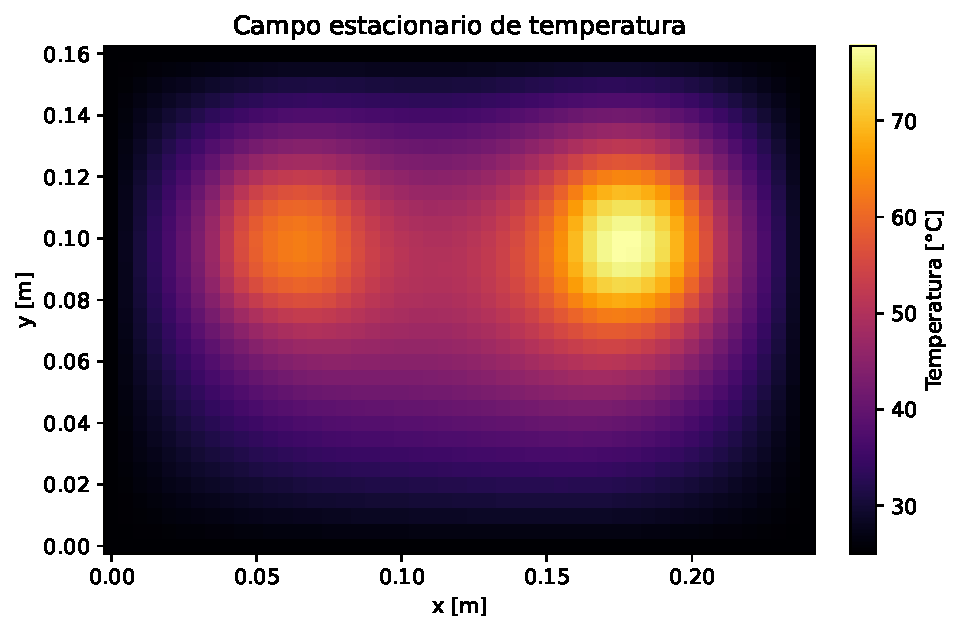
\includegraphics[width=\columnwidth]{../simulacion/figuras/02_mapa_termico.pdf}
\caption{Campo de temperatura estacionario del escenario base.}
\label{fig:mapa-termico}
\end{figure}

\begin{figure}[t]
\centering
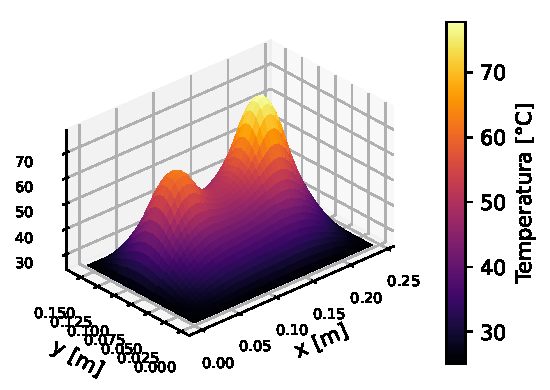
\includegraphics[width=\columnwidth]{../simulacion/figuras/03_superficie_3d.pdf}
\caption{Superficie del mismo campo estacionario presentado en la Figura~\ref{fig:mapa-termico}; la altura y el color representan la temperatura exportada por MATLAB.}
\label{fig:superficie-3d}
\end{figure}

\begin{figure*}[t]
\centering
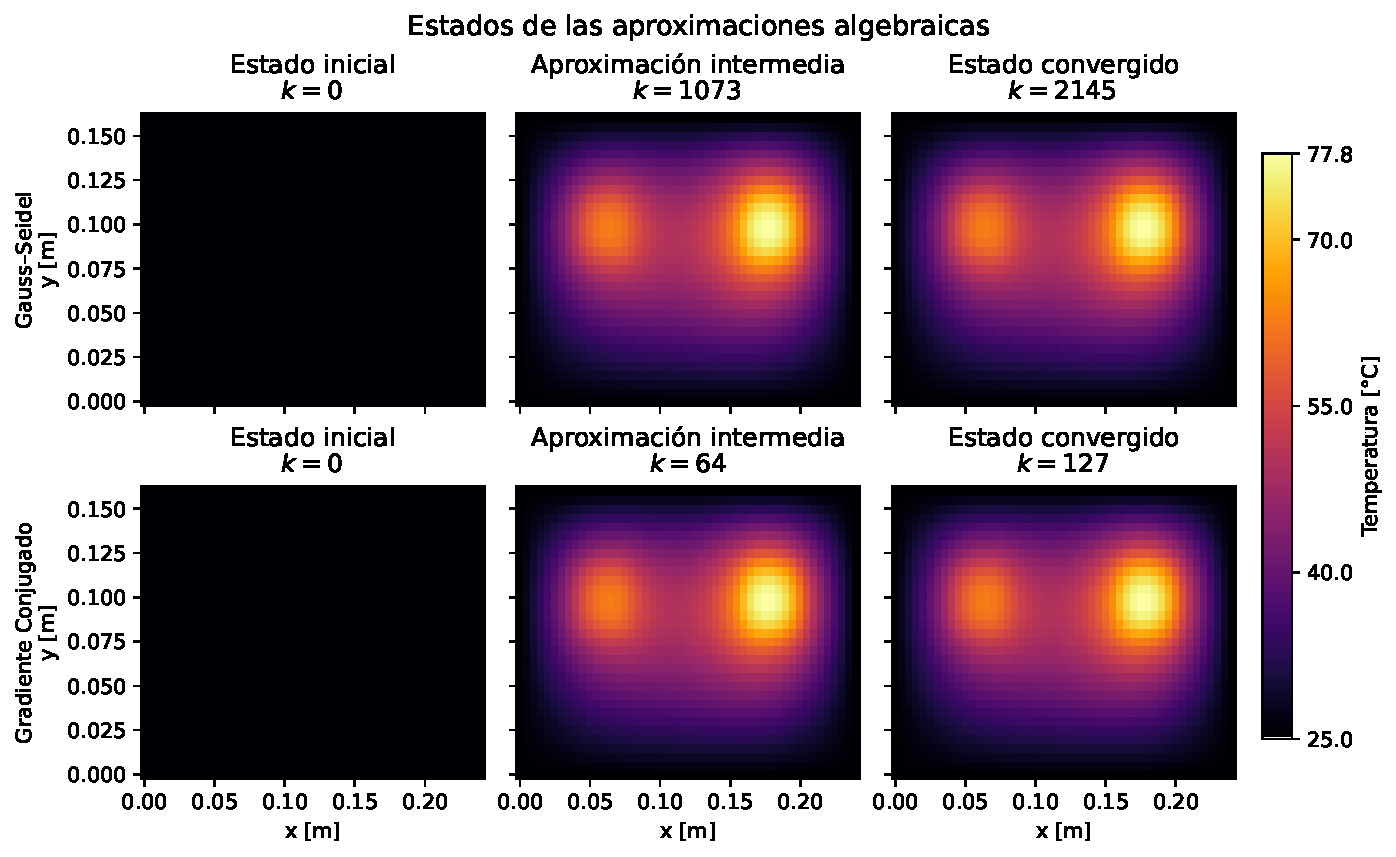
\includegraphics[width=0.94\textwidth]{../simulacion/figuras/04_evolucion_aproximaciones.pdf}
\caption{Estados inicial, intermedio y convergido de las aproximaciones algebraicas de Gauss--Seidel y Gradiente Conjugado. $k$ denota iteraciones del solucionador y no tiempo f\'isico; todos los paneles comparten la misma escala de temperatura.}
\label{fig:aproximaciones}
\end{figure*}

\begin{figure}[t]
\centering
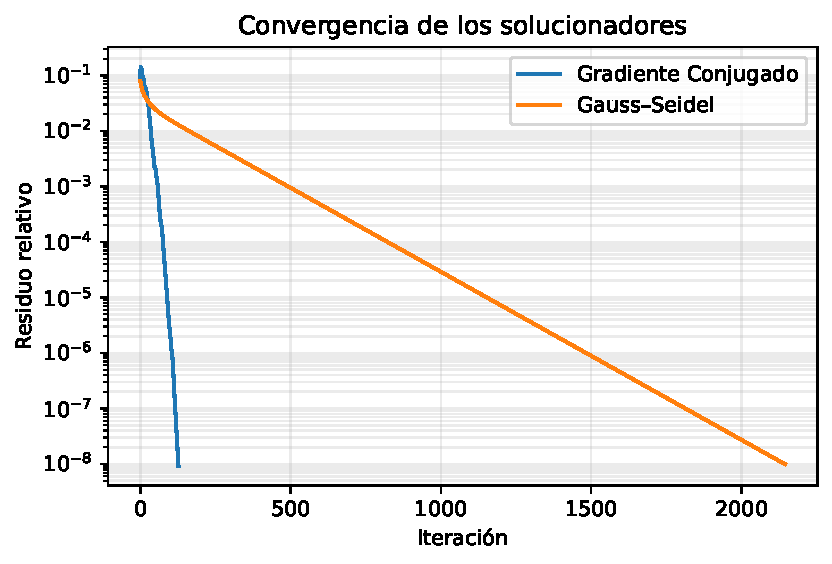
\includegraphics[width=\columnwidth]{../simulacion/figuras/06_residuo_iteraciones.pdf}
\caption{Residuo relativo frente a iteraciones en la malla base.}
\label{fig:residuos}
\end{figure}

\subsection{Refinamiento espacial (objetivo iii)}

Las ocho corridas iterativas de las cuatro mallas convergieron con residuo menor que $10^{-8}$. La Tabla~\ref{tab:refinamiento} muestra que la diferencia nodal m\'axima entre soluciones directas consecutivas se redujo de $0.2385$ a $0.06159$ y $0.01554\ ^\circ$C al duplicar la resoluci\'on. Esta reducci\'on observada es cercana a un factor de cuatro por refinamiento, consistente con el orden espacial esperado en este caso; la diferencia entre mallas no es un error exacto respecto de una soluci\'on anal\'itica. En la malla m\'as fina hay 24,257 inc\'ognitas y el m\'aximo directo es $78.03446\ ^\circ$C.

\begin{table}[t]
\centering
\begin{threeparttable}
\caption{Resultados directos del refinamiento de malla}
\label{tab:refinamiento}
\footnotesize
\begin{tabular}{rrrr}
\toprule
Malla & $N$ & $T_{\max}$ ($^\circ$C) & $\Delta T_m$ ($^\circ$C)\\
\midrule
$25\times17$ & 345 & 77.40879 & 0.23847\\
$49\times33$ & 1457 & 77.75924 & 0.06159\\
$97\times65$ & 5985 & 78.01291 & 0.01554\\
$193\times129$ & 24257 & 78.03440 & --\\
\bottomrule
\end{tabular}
\begin{tablenotes}\footnotesize
\item \textit{Nota.} La diferencia es el m\'aximo absoluto nodal entre la soluci\'on directa de esa malla y la interpolaci\'on bilineal de la siguiente malla m\'as fina. La malla m\'as fina no tiene comparador configurado.
\end{tablenotes}
\end{threeparttable}
\end{table}

En la malla de 24,257 inc\'ognitas, Gauss--Seidel requiri\'o 29,541 iteraciones y una mediana de 52.190 s (desviaci\'on est\'andar 5.502 s); CG requiri\'o 485 iteraciones y una mediana de 0.2043 s (desviaci\'on est\'andar 0.00526 s). La Figura~\ref{fig:costo} resume las medianas e intervalos intercuart\'ilicos de tres repeticiones por malla y m\'etodo. La variaci\'on entre ejecuciones y equipos aconseja interpretar estos cronometrajes como evidencia de la sesi\'on registrada, no como una raz\'on de rendimiento universal.

\begin{figure}[t]
\centering
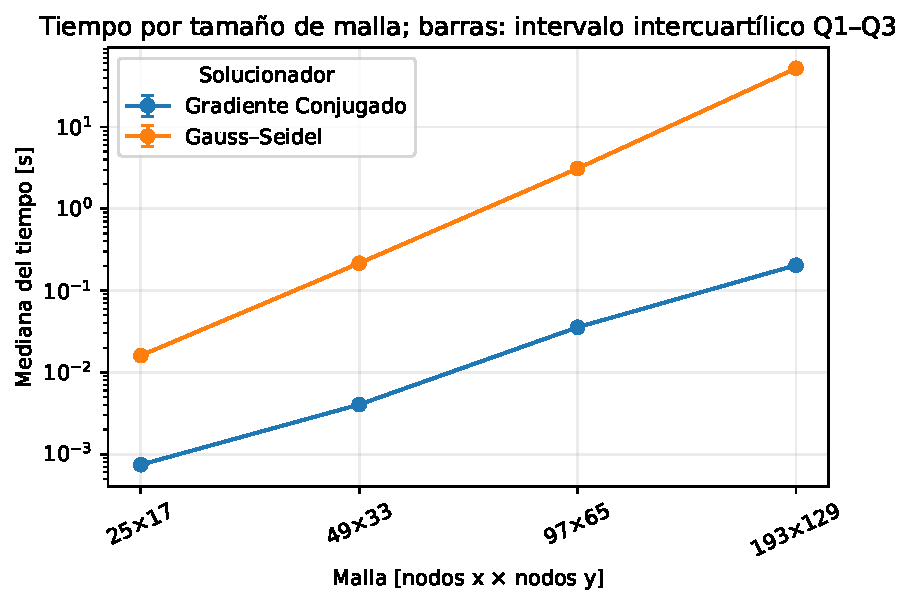
\includegraphics[width=\columnwidth]{../simulacion/figuras/07_costo_refinamiento.pdf}
\caption{Tiempo de soluci\'on por tama\~no de malla; escala vertical logar\'itmica.}
\label{fig:costo}
\end{figure}

\subsection{Sensibilidad de las fuentes (objetivo iii)}

Al variar CPU entre $0$ y $18$ W con GPU fija en $18$ W, $T_{\max}$ aument\'o de $75.0267$ a $79.2360\ ^\circ$C. Al variar GPU entre $0$ y $27$ W con CPU fija en $12$ W, el m\'aximo aument\'o de $58.3511$ a $102.6621\ ^\circ$C. En ambas series se mantuvieron los restantes par\'ametros. La Figura~\ref{fig:sensibilidad} resume los ocho casos y las ubicaciones de los puntos calientes exportadas por MATLAB.

\begin{figure}[t]
\centering
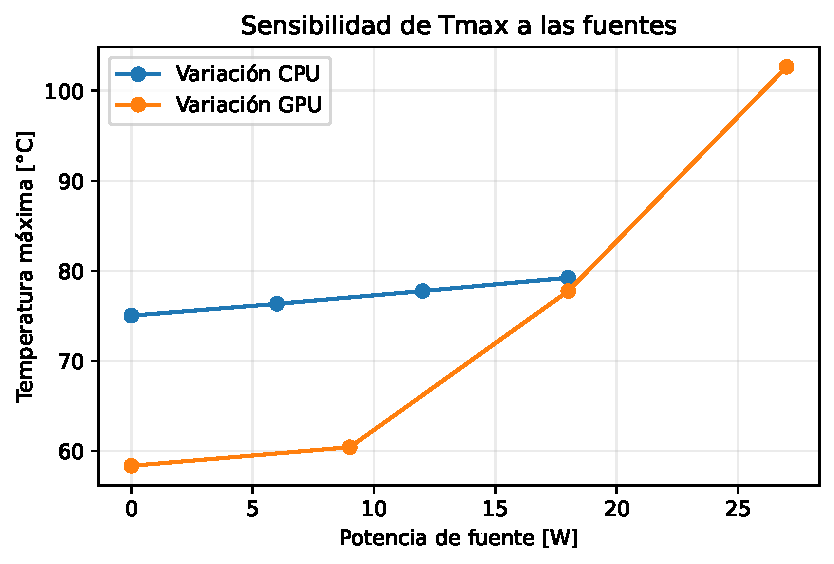
\includegraphics[width=\columnwidth]{../simulacion/figuras/08_sensibilidad_termica.pdf}
\caption{Sensibilidad del m\'aximo de temperatura a la potencia de CPU y GPU.}
\label{fig:sensibilidad}
\end{figure}

\subsection{Estr\'es num\'erico y validaci\'on (objetivos i y iv)}

Para las cuatro tolerancias solicitadas, ambos m\'etodos alcanzaron convergencia. A $10^{-12}$, Gauss--Seidel necesit\'o 3466 iteraciones y obtuvo residuo $9.99\times10^{-13}$; CG necesit\'o 162 iteraciones y obtuvo $8.98\times10^{-13}$. En las pruebas con fuentes multiplicadas por $1000$ y con potencia negativa de CPU, ambos m\'etodos tambi\'en terminaron con estado convergente y residuos menores que $10^{-8}$. El caso extremo y el no f\'isico se reportan solo como pruebas algebraicas, no como escenarios de una laptop. No se observ\'o fallo de convergencia en las corridas registradas.

La verificaci\'on MATLAB document\'o simetr\'ia relativa nula, factorizaci\'on de Cholesky exitosa, error m\'aximo de frontera igual a cero, balance de potencia de $12$ W y $18$ W, y error de linealidad de $4.26\times10^{-14}\ ^\circ$C. El control deliberado con una iteraci\'on m\'axima se identific\'o como \texttt{max\_iterations}; por ello, el estado de no convergencia se detect\'o. El reporte completo y las tablas de cada experimento se conservan en \texttt{simulacion/resultados/} y \texttt{simulacion/pruebas/}.
}
\incluirDesdeAvance{3}{\section{Discusi\'on}

En relaci\'on con el primer objetivo, la discretizaci\'on conserv\'o la potencia integrada de ambas fuentes y produjo una matriz sim\'etrica definida positiva, compatible con los dos solucionadores. Para el segundo objetivo, la Figura~\ref{fig:resultados-base} muestra el m\'aximo dentro de la huella GPU, cuya potencia base fue mayor que la de CPU. La Tabla~\ref{tab:base-solver} cuantifica la respuesta t\'ermica, mientras que estudios de placas reales incorporan capas, interacciones entre componentes y mecanismos de disipaci\'on que aqu\'i se excluyeron \citep{harvest2007devices,moniervinard2015pcb,zhang2024pcb,skadron2003hotspot}. En consecuencia, $77.759239\ ^\circ$C es un resultado del modelo idealizado, no una temperatura operativa medida.

El cuarto objetivo se respondi\'o comparando ambos m\'etodos con la misma $A$, $\mathbf{b}$, condici\'on inicial y tolerancia. La Tabla~\ref{tab:base-solver} y la curva de residuos de la Figura~\ref{fig:resultados-base} muestran que CG alcanz\'o $10^{-8}$ en 127 iteraciones, frente a 2145 de Gauss--Seidel. En la malla m\'as fina, los conteos fueron 485 y 29\,541, respectivamente. La Figura~\ref{fig:estudios-completos} presenta medianas e intervalos intercuart\'ilicos medidos tras calentamiento y en tres repeticiones por configuraci\'on; en esas ejecuciones CG requiri\'o menos tiempo, aunque la dispersi\'on y la dependencia del equipo limitan la generalizaci\'on de los cronometrajes. Esta comparaci\'on concuerda con el uso de CG en sistemas sim\'etricos definidos positivos y con antecedentes de m\'etodos iterativos para Poisson, pero los resultados propios dependen de la matriz, el ordenamiento y la implementaci\'on utilizados \citep{zhang2001,xu2011poisson,oladejo2007tool}.

La Figura~\ref{fig:aproximaciones} muestra que los campos iterativos se construyeron desde el estado inicial uniforme de $25\ ^\circ$C hasta las soluciones convergidas; los paneles intermedios corresponden a iteraciones algebraicas y no a tiempos de calentamiento. La Figura~\ref{fig:resultados-base} permite localizar las fuentes, inspeccionar la geometr\'ia del campo y comparar la reducci\'on del residuo; sus paneles representan el mismo sistema y no constituyen evidencia independiente.

Respecto del tercer objetivo, la Tabla~\ref{tab:refinamiento} muestra que al duplicar la resoluci\'on las diferencias m\'aximas entre soluciones de mallas consecutivas disminuyeron de $0.23847$ a $0.06159$ y $0.01554\ ^\circ$C. La tendencia, cercana a una reducci\'on por cuatro, es compatible con el comportamiento esperado de diferencias centrales de segundo orden en las mallas evaluadas; no equivale a un error exacto porque no se dispone de soluci\'on anal\'itica para las fuentes discontinuas y la malla m\'as fina carece de una malla de referencia superior. La Figura~\ref{fig:estudios-completos} completa el an\'alisis al mostrar el aumento del costo computacional al crecer el sistema. La interpretaci\'on es consistente con an\'alisis de esquemas para Poisson y trabajos de refinamiento, sin atribuir sus garant\'ias te\'oricas a esta prueba particular \citep{settle2013compact,chen2007supra,raeli2018hierarchical,batty2017cell}.

La Figura~\ref{fig:estudios-completos} resume las ocho configuraciones de fuentes y muestra un aumento del m\'aximo al elevar por separado la potencia de CPU o GPU. La ecuaci\'on discreta es lineal respecto de las potencias cuando se mantienen las propiedades y las fronteras; sin embargo, $T_{\max}$ es el m\'aximo global del campo y puede cambiar de ubicaci\'on, por lo que la curva no tiene que ser una recta con pendiente constante. La sensibilidad orienta el an\'alisis de esta idealizaci\'on y no sustituye los modelos multicapa, transitorios y con disipaci\'on que se aplican a placas reales \citep{chung2001materials,zheng2021advances,harvest2007devices,moniervinard2015pcb}.

La verificaci\'on complementaria confirm\'o residuo relativo menor que la tolerancia, concordancia cercana con la referencia directa, simetr\'ia, definitud positiva, cumplimiento de frontera y conservaci\'on de la potencia discretizada. Las pruebas de tolerancia, potencia extrema y potencia negativa evaluaron el comportamiento algebraico; las dos pruebas de potencia no describen condiciones f\'isicas. La diferencia entre soluci\'on iterativa y referencia directa estima el error algebraico, mientras que la comparaci\'on entre mallas caracteriza el cambio espacial. Ninguna mide el error de modelaci\'on f\'isica, que requerir\'ia comparar con una placa y condiciones experimentales documentadas. Las soluciones de verificaci\'on para s\'olidos con calentamiento parcial y los modelos num\'ericos alternativos de conducci\'on proveen referentes metodol\'ogicos, pero sus geometr\'ias y condiciones de frontera no validan directamente THERMOPLATE \citep{beck2004verification,akeremale2020finite,reutskiy2016meshless,deng2017high}.
}
\incluirDesdeAvance{4}{\section{Conclusiones}

El objetivo general se cumplió al formular y resolver numéricamente la conducción estacionaria en la placa idealizada y comparar los solucionadores sobre el mismo sistema discretizado. En respuesta al primer objetivo específico, las diferencias centrales condujeron a una matriz dispersa simétrica definida positiva, con condiciones de Dirichlet y una discretización que conservó las potencias prescritas. Para el escenario base del segundo objetivo, la solución directa produjo $T_{\max}=77.7592\ ^\circ$C; con residuo relativo menor que $10^{-8}$, Gauss--Seidel convergió en 2145 iteraciones y Gradiente Conjugado en 127. Respecto del tercer objetivo, el refinamiento redujo las diferencias nodales entre mallas sucesivas y el aumento de potencia de las fuentes elevó el máximo térmico. Para el cuarto, ambos métodos alcanzaron la tolerancia y coincidieron estrechamente con la referencia directa, mientras CG requirió menos iteraciones y presentó menores tiempos medianos en las corridas registradas.

La contribución del estudio es una implementación reproducible que separa el error algebraico del cambio espacial y de las simplificaciones físicas, y que compara los métodos con repeticiones de tiempo y exportaciones trazables. El alcance se limita a una placa homogénea bidimensional en estado estacionario, con fuentes uniformes idealizadas y temperatura de contorno fija; por ello, los resultados no predicen temperaturas de una laptop real ni incluyen convección, radiación, transitorios o materiales multicapa. Como continuación, convendría incorporar propiedades y geometría de una placa documentada, condiciones de disipación medidas y un modelo transitorio, y contrastar las predicciones con datos experimentales antes de atribuirles valor de diseño.
}

% ============================================================
% REFERENCIAS
% ============================================================

% Solo se imprimen las fuentes citadas mediante \citep o \citet.
\prepararReferenciasAPA
\printbibliography

% Los anexos se colocan despues de las referencias y solo en el avance final.
\incluirDesdeAvance{4}{\clearpage
\appendix
\section{Anexos}

\subsection{Repositorio de implementaci\'on y reproducibilidad}

El c\'odigo fuente computacional utilizado en el estudio est\'a disponible en el repositorio p\'ublico \href{https://github.com/Pepe17xd/Metodos-Numericos}{https://github.com/Pepe17xd/Metodos-Numericos}. All\'i se encuentran las implementaciones MATLAB \texttt{.m} y los cuadernos ejecutables \texttt{.mlx}, los scripts de visualizaci\'on Python, las configuraciones, las pruebas automatizadas y las instrucciones para reproducir las simulaciones. El campo de temperatura, los historiales de convergencia y las tablas de experimentos se exportan desde MATLAB; Python lee esos resultados para generar las figuras, sin resolver de nuevo el modelo.

Las instrucciones para configurar MATLAB R2025a, instalar las dependencias de Python, ejecutar las pruebas y regenerar los resultados y visualizaciones se describen en el archivo \texttt{README.md} del repositorio. Se incluyen las fuentes LaTeX del paper, una instant\'anea de las exportaciones MATLAB y las figuras generadas desde esos datos; todo puede regenerarse con el flujo documentado.
}

\end{document}
